
%(BEGIN_QUESTION)
% Copyright 2012, Tony R. Kuphaldt, released under the Creative Commons Attribution License (v 1.0)
% This means you may do almost anything with this work of mine, so long as you give me proper credit

A large natural gas compressor takes in gas from three different sources, ``knocks out'' any liquid that might be entrained in the gas, and then boosts the pressure of that gas for transport through miles of piping:

$$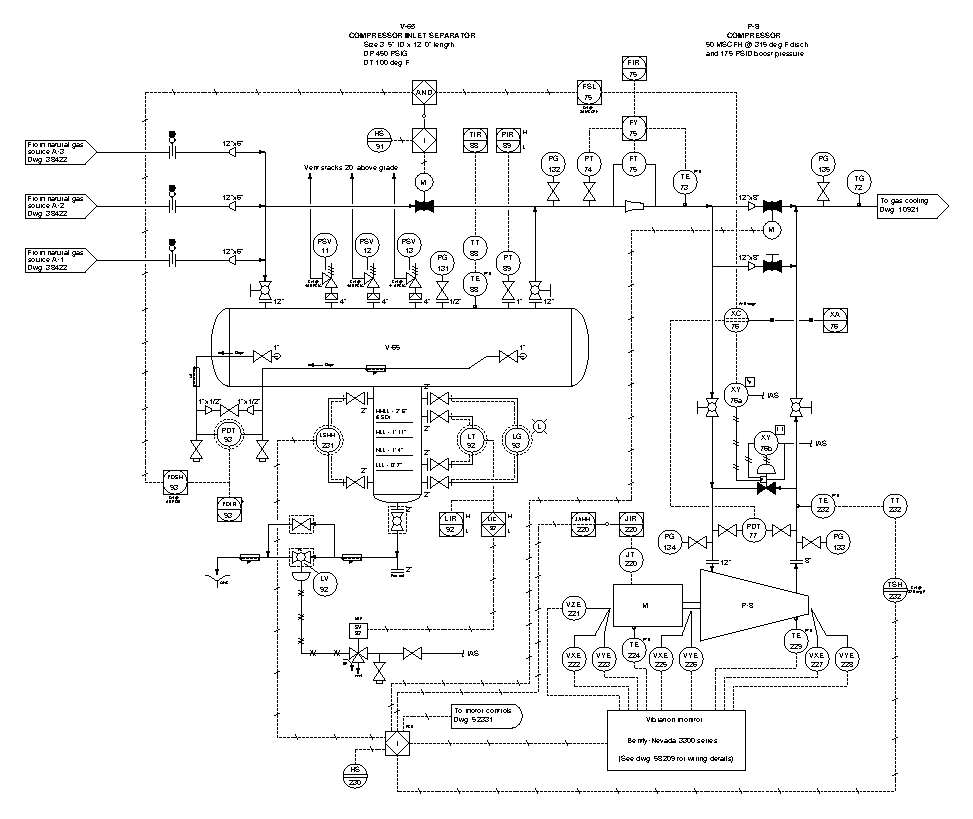
\includegraphics[width=15.5cm]{i0003rx01.eps}$$

Flowmeter FT-75 has been in service for many years, but unfortunately does not provide good enough turndown for operations' needs when the compressor is operated at a fraction of its rated capacity.  Engineers are debating what type(s) of flowmeter might be used to replace FT-75.

\vskip 10pt

First, explain what ``turndown'' means in the context of this flowmeter, and explain why this particular type of flowmeter might not provide good enough turndown.

\vskip 10pt

Brainstorm some different flow-sensing technologies, and then determine whether or not each one of them could be applied here.

\underbar{file i00978}
%(END_QUESTION)





%(BEGIN_ANSWER)

Turndown refers to the ratio of minimum to maximum flow rate that may be accurately sensed by a particular flowmeter while remaining within acceptable limits of measurement error.  Differential-pressure based flowmeters such as this venturi tube typically exhibit turndown ratios of only 4:1 (or sometimes worse) due to measurement uncertainties caused by uneven impulse line liquid heights, DP sensor calibration error, etc.  The nonlinear nature of the flow/pressure relationship is the root of this problem.

\vskip 10pt

\begin{itemize}
\item{} {\bf Positive displacement} -- Probably not suitable, due to possible particulate matter in the gas stream, and the high volume of flow expected.  High volumes would require either a huge flowmeter, or would induce undue wear and tear in the fast-moving meter mechanism.
\vskip 10pt
\item{} {\bf Turbine} -- Possibly suitable.  Pressure and temperature compensation would both be necessary to calculate true volumetric flow rate, however.
\vskip 10pt
\item{} {\bf Vortex} -- Possibly suitable, so long as the minimum flow rate exceeded the low-flow cutoff point for the flowmeter.  If minimum flow could be ensured, pressure and temperature compensation would both be necessary to calculate true volumetric flow rate.
\vskip 10pt
\item{} {\bf Magnetic} -- Definitely unsuitable, due to non-conductivity of vapors in general.
\vskip 10pt
\item{} {\bf Ultrasonic} (Doppler) -- Definitely unsuitable, due to lack of objects in flow stream to reflect sound waves. 
\vskip 10pt
\item{} {\bf Ultrasonic} (transit time) -- Possibly suitable.  Pressure and temperature compensation would both be necessary to calculate true volumetric flow rate, however.
\vskip 10pt
\item{} {\bf Coriolis} -- Definitely suitable, but most likely too expensive to consider for this application.
\vskip 10pt
\item{} {\bf Thermal mass} -- Possibly suitable, so long as the specific heat of the natural gas was relatively stable over time.  If not, compensation may be possible using a gas chromatograph to analyze the composition of the natural gas stream (gas chromatography is typically done anyway in the gas pipeline industry to determine the chemical heating value of the gas!).
\end{itemize}

 
%(END_ANSWER)





%(BEGIN_NOTES)


%INDEX% Process: gas compressor inlet separator (realistic P&ID shown)

%(END_NOTES)


